\chapter{Informační systém pro správu závěrečných prací}

Téma bakalářská práce se zaměřuje na analýzu, návrh a~implementaci informačního systému pro správu bakalářských a~diplomových prací. Informační systém slouží především firmě Red Hat jako nástroj pro zadání, kontrolu a~schvalování závěrečných prací vypsaných na partnerských fakultách. Systém zároveň poskytuje rozhraní pro studenty, kteří se mohou přihlašovat k~tématům, komentovat jednotlivá témata a~závěrečné práce. Dále k~systému přistupuje vedoucí, který schvaluje přihlášení k~tématům a~spravuje stav závěrečných prací. Systém je veřejný a~návštěvníci tak mají možnost procházet jednotlivá témata a~závěrečné práce, dále se mohou registrovat na základě fakultního e-mailu. Hlavní strana systému slouží jako přehled nejnovějších aktivit v~systému.

Mým úkolem je vytvořit grafickou podobu uživatelského rozhraní a tento návrh integrovat do systému.

\section{Popis požadavků na systém}

Systém eviduje---

\begin{itemize}
    \item Témata
    \item Závěrečné práce
    \item Uživatele
    \item Univerzity
    \item Přihlášky
\end{itemize}

Témata popisují cíl práce, mohou být vypsány pro více studentů. Systém umožňuje témata vypisovat, editovat a mazat. Témata evidují---

\begin{itemize}
    \item Seznam přihlášených studentů
    \item Seznam univerzit, na kterých je téma vypsáno
    \item Seznam vedoucích
    \item Seznam závěrečných prací, které byly na základě tématu vypsány
\end{itemize}

Ke každé závěrečné práci se smí přihlásit pouze jeden student. Systém umožňuje práce vytvářet (na základě tématu), editovat a mazat. Každá závěrečná práce eviduje---

\begin{itemize}
    \item Studenta přihlášeného k práci
    \item Téma, ze kterého byla práce vypsána
    \item Univerzitního vedoucího práce
    \item Typ závěrečné práce -- bakalářská nebo diplomová práce
    \item Stav závěrečné práce -- přihlášená, dokončená, neúspěšná a odložená
\end{itemize}

V systému tak existuje několik uživatelských rolí, které se liší v přístupových právech. Každý registrovaný uživatel je automaticky student. Práva uživatelských rolí---

\begin{itemize}
    \item Návštěvníci -- mohou procházet jednotlivá témata, závěrečné práce a registrovat se dle fakultního e-mailu.
    \item Studenti -- mohou se přihlašovat k tématům, spravovat vlastní závěrečné práce a diskutovat k jednotlivým tématům a závěrečným pracím.
    \item Univerzitní vedoucí -- jedná se o vedoucího na dané univerzitě, může vytvářet závěrečné práce, schvaluje přihlášky a má právo přispívat v diskuzích.
    \item Vedoucí -- na rozdíl od univerzitního vedoucího navíc vytváří témata závěrečných prací.
    \item Správce -- může spravovat většinu obsahu, přidávat univerzity a uživatele.
\end{itemize}

\section{Analýza cílové skupiny}

Cílová skupina uživatelů přistupujících k systému je velmi úzce zaměřená. Největší část návštěvníků tvoří studenti z technicky zaměřených oborů. Tato skupina je dána typem závěrečných prací, pro které je systém primárně určen---jedná se o témata z IT oboru. Příklady některých univerzit, které jsou v systému registrovány---

\begin{itemize}
    \item Masarykova univerzita
    \item Vysoké učení technické v Brně
    \item České vysoké učení technické v Praze
\end{itemize}

Systém je určen především pro studenty v posledních ročnících bakalářského nebo magisterského studia a jejich vedoucí.

\section{Základní layout}

Rozhodl jsem se používat tři základní layouty stránky, přičemž dva se liší pouze prohozením postranního panelu a obsahové části. Primární layout (viz obrázek \ref{img:layout1}) tvoří---

\begin{itemize}
    \item Navigační panel -- nachází se v záhlaví stránky a obsahuje hlavní informace o přihlášeném uživateli, vyhledávač a logotyp.
    \item Navigační menu -- slouží jako primární navigace na stránce.
    \item Levý sloupec s hlavním obsahem -- je určený pro seznam témat, závěrečných prací a jejich popis. Dále může obsahovat odevzdávárnu souborů a komentáře.
    \item Pravý sloupec s vedlejším obsahem -- slouží jako přehled informací o daném tématu nebo závěrečné práci. Dále může obsahovat nástroje pro správu témat (popř. závěrečných prací) nebo filtry.
\end{itemize}

Sekundární layout představuje kostru uživatelského profilu a profilu univerzity. Na rozdíl od primárního layoutu je sloupec s vedlejším obsahem přemístěn na levou část stránky. Tvoří ho---

\begin{itemize}
    \item Navigační panel
    \item Navigační menu
    \item Levý sloupec s vedlejším obsahem -- obsahuje podrobnější informace o uživateli včetně profilového obrázku.
    \item Pravý sloupec s hlavním obsahem -- slouží jako obecný přehled vedených závěrečných prací, vlastních prací a aktivity uživatele v systému.
\end{itemize}

Poslední layout je speciálně navržený pro formuláře. Obsahuje pouze nejnutnější elementy a je tvořen z jednoho sloupce---

\begin{itemize}
    \item Navigační panel
    \item Hlavní sloupec -- určený pro formulářová pole.
\end{itemize}

\begin{figure}[htbp]
    \centering
    \includegraphics[width=\textwidth]{images/main-layout.png}
    \caption{Výsledný drátěný model -- profil diplomové práce.}
    \label{img:layout1}
\end{figure}

Minimální šířka všech stránek je 1040$px$ -- při nižších hodnotách je uživatel nucen horizontálně skrolovat. Tuto šířku jsem zvolil s ohledem na aktuální podíl populárních rozlišení u displejů zařízení, který v současnosti z více než 90\% tvoří rozlišení větší než 1024$\times$768$px$\footnotemark[1].

\footnotetext[1]{\url{http://gs.statcounter.com/\#resolution-CZ-monthly-201203-201303}}

\section{Grafický návrh}

Přesto, že nebyly kladeny žádné větší nároky na dodržení vizuálního stylu společnosti Red Hat, rozhodl jsem se z něj čerpat alespoň částečně především co se týče barevnosti.

\subsection{Písmo}

Ještě relativně nedávno byly designeři při volbě písma pro webové aplikace omezeni na několik málo základních fontů, které byly ve většině případů přítomny na klientských počítačích -- například Arial, Times New Roman, Georgia nebo Courier Sans. Díky nového CSS pravidla \texttt{@font-face} je možné používat i fonty, které nejsou na klientských počítačích nainstalovány.

Již na počátku tvorby jsem se rozhodl používat pro nadpisy lineárně serifové písmo s rovnými serify\footnotemark[1]. Volba písma je značně omezená především pro nutnost podpory české znakové sady. První volbou bylo písmo Sanchez\footnotemark[2], které jsem však později zavrhl z důvodu špatné optimalizace pro webové prohlížeče. Nakonec jsem zvolil písmo Museo Slab\footnotemark[3], které navrhl designer Jan Buivenga.

\footnotetext[1]{Viz klasifikace písma podle Jana Solpery.}
\footnotetext[2]{\url{http://www.myfonts.com/fonts/latinotype/sanchez/}}
\footnotetext[3]{\url{http://www.myfonts.com/fonts/exljbris/museo-slab/}}

\begin{figure}[htbp]
    \centering
    \includegraphics[width=\textwidth]{images/museo.pdf}
    \caption{Museo Slab 500}
    \label{img:museo}
\end{figure}

Jako primární písmo jsem se rozhodl použít velmi rozšířený Arial. Jedná se o bezpatkový grotesk, který je již od počátku součástí všech verzí Microsoft Windows. Arial bývá často kritizován pro svou podobnost s Helveticou, přesto se však jedná o velmi dobře čitelný a vysoce optimalizovaný font.

\subsection{Piktogramová řada}

Jako sadu ikonek jsem zvolil Font Awesome\footnotemark[1], který byl primárně navržený pro webový rámec Twitter Bootstrap. Samotná piktogramová řada je vedena pod licencí CC BY 3.0, je tedy možné používat řadu samostatně.

\footnotetext[1]{\url{http://fortawesome.github.io/Font-Awesome}}

\subsection{Typografie}

Jako základní velikost písma jsem zvolil 16$px$, díky čemuž je text dobře čitelný i na monitorech s hustším PPI. Vzhledem k větší střední výšce písma Arial jsem se rozhodl použít vyšší hodnotu řádkového prokladu, aby i rozsáhlejší části textu nepůsobily příliš sevřeně.

Nadpisy první až čtvrté úrovně jsou vysázeny písmem Museo Slab s maximální velikostí 34$px$, která je užita výhradně pro názvy témat a závěrečných prací.

Velikost okrajů primárního sloupce s obsahem jsem se rozhodl nastavit na 30$px$, čímž je zajištěn dostatečný prostor pro jednoduchou orientaci mezi odstavci a jsou tak jasně odlišeny bloky textu.

\subsection{Barevnost}

Vizuální styl společnosti Red Hat se orientuje v barvách bílé, černé a červené. Rozhodl jsem se použít světlejší barvy pro navození klidnějšího dojmu a snížení kontrastu, neboť příliš vysoký kontrast může působit dráždivě a není podle mě příliš vhodný pro stránky určené primárně pro správu závěrečných prací.

V grafickém návrhu používám osm stupňů šedi a dva stupně červené barvy. Několik dalších barev je použito výjimečně například pro zvýraznění aktivních kategorií nebo pro systémové zprávy a upozornění.

\begin{figure}[htbp]
    \centering
    \includegraphics[width=\textwidth]{images/barvy.pdf}
    \caption{Základní barvy použité v uživatelském rozhraní.}
    \label{img:colors}
\end{figure}

\begin{figure}[htbp]
    \centering
    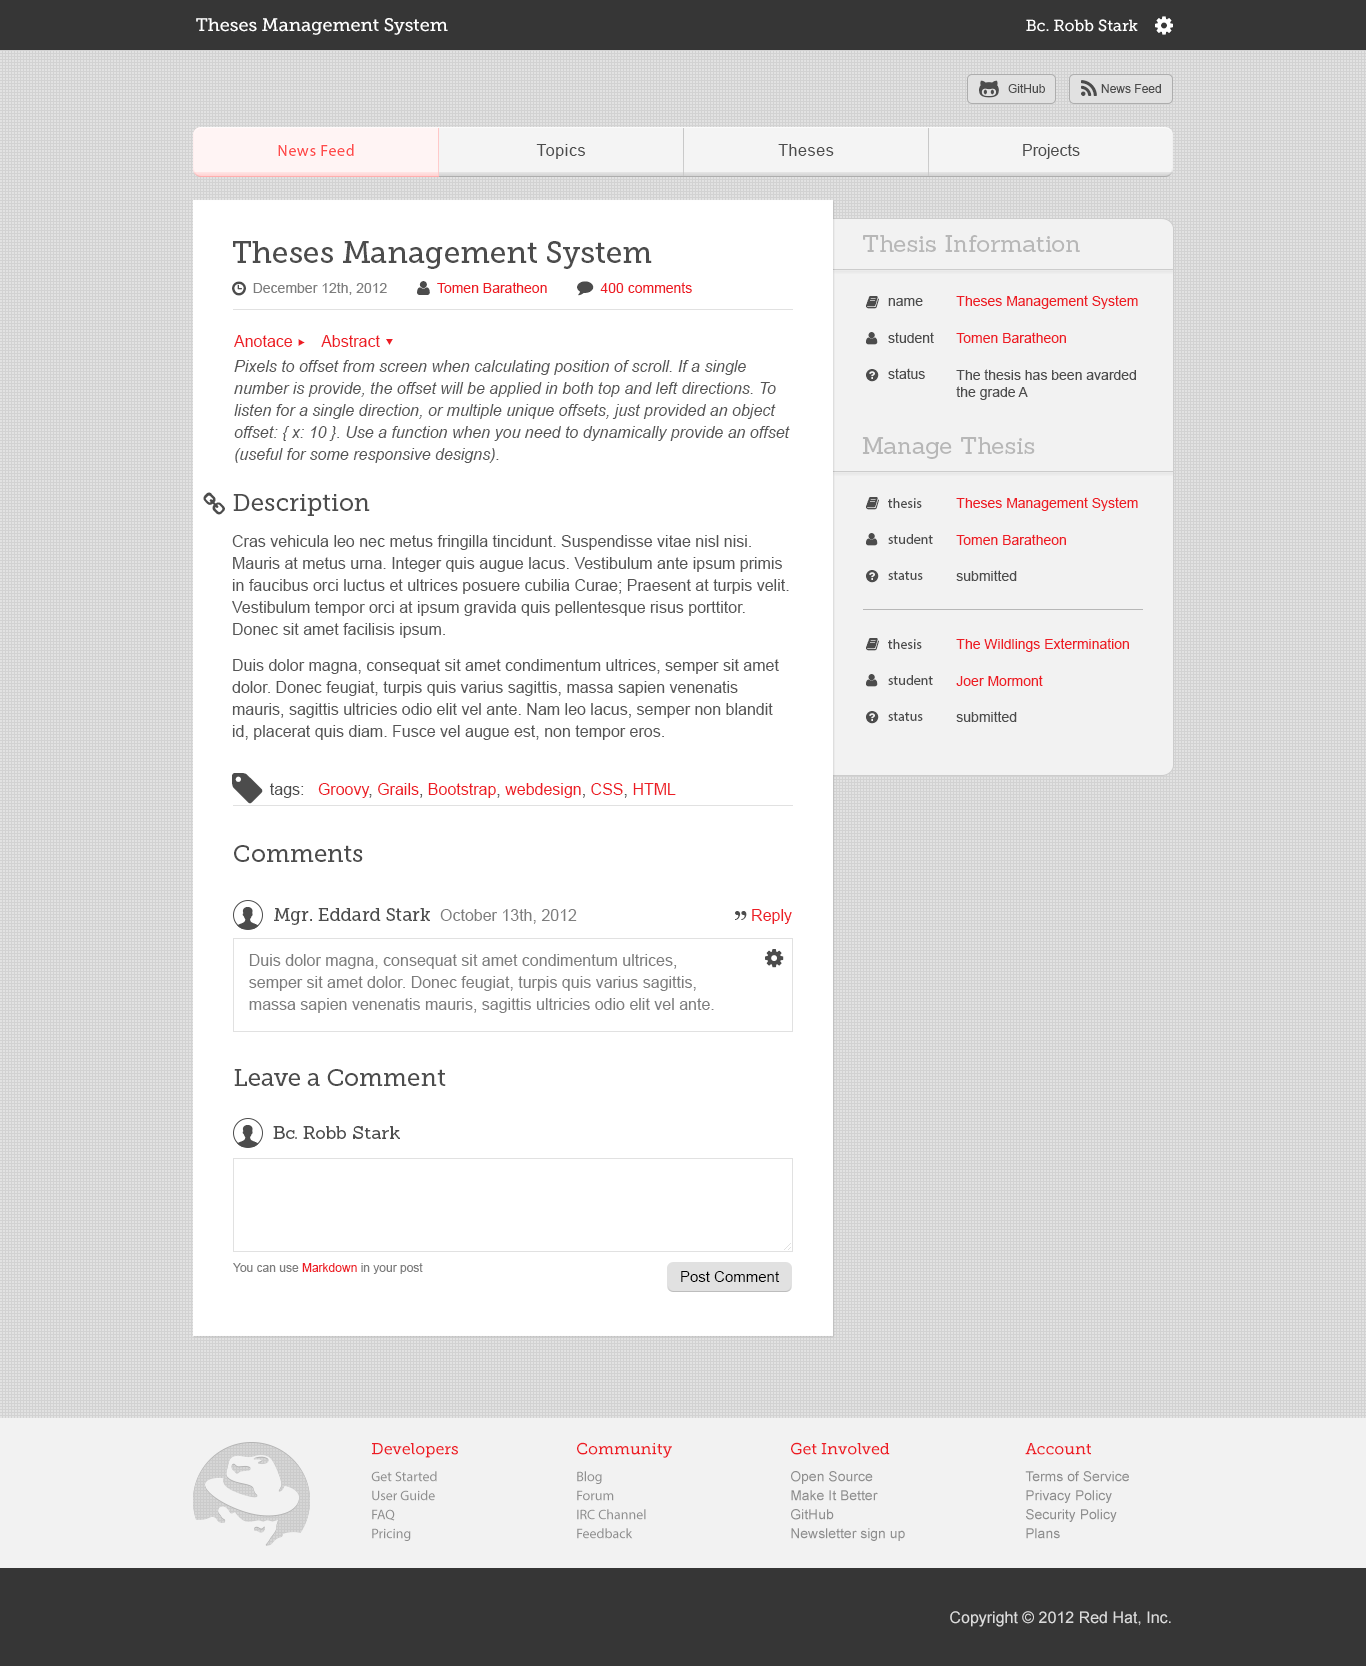
\includegraphics[width=\textwidth]{images/design.png}
    \caption{Výsledný grafický návrh -- profil diplomové práce.}
    \label{img:design}
\end{figure}

\section{Použité webové technologie}

Prezentační vrstva systému využívá následující technologie, knihovny a webové rámce---

\begin{enumerate}
    \item HTML~5 (viz kapitola~\ref{sec:html})
    \item CSS~3 (viz kapitola~\ref{sec:css})
    \item LESS (viz kapitola~\ref{sec:less})
    \item JavaScript\footnotemark[1]
    \item Twitter Bootstrap (viz kapitola~\ref{sec:bootstrap})
    \item GSP (viz kapitola~\ref{subsec:gsp})
\end{enumerate}

Zatímco ve čtvrté kapitole jsem se věnoval specifikaci několika výše jmenovaných technologií, nyní se zaměřím na jejich použití v našem systému. Vzhledem k zaměření systému však není potenciál všech použitých technologií plně využit (jde zejména o HTML~5 standard).

\footnotetext[1]{JavaScript je skriptovací dynamicky typovaný jazyk určen primárně pro rozšíření HTML dokumentu o dynamické chování na straně klienta.}

\subsection{HTML~5}

Velká část HTML~5 je v současné době všemi moderními prohlížeči podporována a je tak již možné mnoho novinek volně používat. Aplikace implementuje v zásadě jen některé nové HTML atributy a sémantické elementy. V budoucnu je však možné aplikaci rozšířit o další novinky a vylepšení, které tento nový standard přináší.

\subsection{CSS~3}

Nové vlastnosti a selektory využívám v systému hojně, neboť umožňují jednak velkou část webu vytvořit bez použití rastrových obrázků, dále zvyšují čistotu kódu a pomáhají zachovat jednoduchost stránky z hlediska její struktury.

Mezi jednu z předních výhod CSS~3 patří revoluce v podobě pravidla \texttt{@font-face}, která umožňuje definici vlastních fontů. Tímto je zároveň umožněno použití sady piktogramů ve formě fontu, díky čemuž odpadá nutnost práce s rastrovou sadou ikonek. Tyto možnosti uplatňuji užitím fontu Awesome jako sady piktogramů a fontu Museo Slab pro čtyři úrovně nadpisů.

\begin{example}
    \centering
    \begin{lstlisting}
/* Definice fontu v CSS */
.icon-rss:before { content: "\f09e"; }
    \end{lstlisting}
    \begin{lstlisting}
<!-- Pouziti v HTML dokumentu -->
<a id="news" href="${createLink(uri: '/rss')}">
    <i class="icon-rss"></i>
    <g:message code="feed.news.label"/>
</a>
    \end{lstlisting}
    \caption{Použití fontu Awesome -- odkaz na RSS čtečku.}
    \label{example:awesome}
\end{example}

\subsection{Twitter Bootstrap}

Díky Twitter Bootstrapu je návrh jednotlivých HTML dokumentů konzistentní a lépe udržovatelný. Zároveň je tak docíleno vyšší podpory webovými prohlížeči, přičemž jsou dodržovány osvědčené postupy a doporučení.

Použití Bootstrapu mě zbavilo nutnosti trávit nadměrné množství času optimalizací aplikace pro webové prohlížeče, zároveň mi rámec nabídl mnoho nástrojů a předdefinovaných komponent, které urychlili vývoj prezentační vrstvy aplikace.

Vzhledem k tomu, že se grafický návrh vyvíjeného systému značně liší od vizuálního stylu Bootstrapu, bylo potřeba některé součásti upravovat. Tento úmysl je běžný pro mnoho aplikací, které používají nějaký webový rámec pro tvorbu uživatelského rozhraní. S tímto problémem se lze vypořádat částečným přepsáním zdrojového kódu webového rámce podle vlastních potřeb. Takový postup však není doporučován, neboť znemožňuje rámec později aktualizovat. Rozhodl jsem se tedy pro řešení, které znázorňuje adresářová struktura na obrázku \ref{fig:tree}, kde---

\begin{itemize}
    \item adresář \texttt{bootstrap} obsahuje zdrojové soubory Twitter Bootstrapu
    \item soubor \texttt{bootstrap.less} obsahuje importy použitých komponent Bootstrapu a vlastní definované CSS styly, jež musí být umístěny hierarchicky na konci souboru
    \item soubor \texttt{variables.less} je určený pro deklaraci proměnných
    \item soubor \texttt{main.less} slouží pro definici vlastních stylů
\end{itemize}


\begin{figure}
    \dirtree{%
    .1 less.
    .2 bootstrap.
    .3 alerts.less.
    .3 ....
    .2 bootstrap.less.
    .2 variables.less.
    .2 main.less.
    .2 ....
    }
    \caption{Stromová struktura adresáře s CSS styly.}
    \label{fig:tree}
\end{figure}

\subsection{LESS}

Použití preprocesoru LESS zpřístupnilo mnoho konstrukcí, které v čistém CSS z důvodu zachování formální čistoty jazyka chybí. Díky LESS je stylopis přehlednější, kratší a organizovanější. Chceme-li například změnit barvu odkazů nebo odstranit podtržení, stačí tak učinit na jediném místě v kódu.

Pro eliminaci neúmyslného přepsání CSS stylů definovaných Bootstrapem jsem v systému zavedl konvenci pro pojmenování vlastních tříd a identifikátorů. Každá vlastní třída obsahuje prefix \texttt{tms-}, tedy například definované tlačítka jsou v systému označovány třídou \texttt{.tms-btn}, naopak v Bootstrapu pouze \texttt{.btn}.

Vlastní CSS styly jsou definovány v souborech---

\begin{itemize}
    \item \texttt{main.less} -- určený pro formátování selektorů, tříd, identifikátorů a definici mixinů, zatímco proměnné jsou deklarovány v souboru přejatém od Bootstrapu (\texttt{variables.less})
    \item \texttt{fonts.less} -- definice fontů používaných v systému
    \item \texttt{taggy.less} -- CSS styly přídavného modulu pro podporu tagů
    \item \texttt{fineuploader.less} -- CSS styly přídavného modulu pro podporu nahrávání souborů
\end{itemize}

\subsection{GSP}
\label{subsec:gsp}

Hlavní funkce systému jsou napsané v programovacím jazyce Groovy za použití platformy Grails. Výchozí jazyk této platformy určený pro popis prezentační vrstvy systému je GSP (\textit{Groovy Server Pages}), což je jazyk inspirovaný JSP (\textit{JavaServer Pages}) speciálně navržený pro dynamické zpracování HTML dokumentů. Přestože syntaxe GSP vychází z XML, nejedná se o XML validní stránky.

GSP umožňuje aplikovat dynamické chování dokumentu jednak zasazením samotného Groovy kódu mezi bloky \texttt{<\% ... \%>} (jedná se však o nedoporučený postup) nebo použitím GSP elementů. V aplikaci používáme druhý způsob, mezi jehož největší nevýhodu patří relativně vysoká nepřehlednost.

V ukázce \ref{example:parent} lze vidět příklad GSP stránky. Tato stránka slouží jako layout pro \uv{potomky} (t.j. stránky, které takto definovaný dokument rozšiřují).

\begin{example}
    \centering
    \begin{lstlisting}
<html>
  <head>
    <title><g:layoutTitle /></title>
    <g:layoutHead />
  </head>
  <body>
    <div class="span9">
        <g:layoutBody />
    </div>
  </body>
</html>
    \end{lstlisting}
    \caption{Rodič -- \texttt{light.gsp}.}
    \label{example:parent}
\end{example}

Každý potomek je definován uvedením rodiče v meta elementu (jako v ukázce \ref{example:child}), přičemž na místo elementu \texttt{<g:layoutBody />} je vykresleno tělo potomka, element \texttt{<g:layoutHead />} je nahrazen hlavičkou a \texttt{<g:layoutTitle />} titulkem potomka.
\begin{example}
    \centering
    \begin{lstlisting}
<html>
  <head>
    <meta name="layout" content="light">
    ...
  </head>
  <body>
    ...
  </bodu>
</html>
    \end{lstlisting}
    \caption{Potomek stránky \texttt{light.gsp}.}
    \label{example:child}
\end{example}
